% Capítulo 2 - Fundamentação Teórica (versão enxuta): FPGAs e MLP em FPGA
\section{\textit{Field-Programmable Gate Arrays} (FPGAs)}
\label{sec:FPGA}

Os FPGAs são circuitos integrados cuja lógica interna é configurada após a fabricação. Diferem dos circuitos integrados de aplicação específica (\textit{Application-Specific Integrated Circuits}, ASICs), que executam uma função fixa, e dos processadores, que executam instruções em sequência: no FPGA, o algoritmo é descrito em uma linguagem de descrição de \textit{hardware} (\textit{Hardware Description Language}, HDL), como VHDL ou Verilog, e convertido em um circuito digital dedicado, com operações paralelas e latência determinística \cite{kuon2008fpga,trimberger2015three}. Essa combinação de reconfigurabilidade, paralelismo e baixa latência faz do FPGA uma plataforma adequada à aquisição e ao processamento de sinais em alta taxa e à inferência de redes neurais embarcadas \cite{Shawahna2019}.

\subsection{Arquitetura e recursos}

Um FPGA é uma matriz de blocos lógicos ligados por uma rede de interconexão programável e complementados por blocos dedicados (Figura~\ref{fig:FPGA_internal_architeture}) \cite{langhammer2014design}. Os recursos que limitam um projeto, e que são relatados neste trabalho, são:
\begin{itemize}
	\item \textbf{LUTs e \textit{flip-flops}}: os blocos lógicos configuráveis (\textit{Configurable Logic Blocks}, CLBs) contêm tabelas de consulta (\textit{Look-Up Tables}, LUTs), que implementam funções lógicas arbitrárias de poucas entradas, e \textit{flip-flops}, que armazenam estado;
	\item \textbf{BRAM}: blocos de memória interna, usados como \textit{buffers} e para guardar coeficientes e dados intermediários sem acesso à memória externa;
	\item \textbf{DSP}: blocos aritméticos dedicados a multiplicação e acumulação (\textit{multiply-accumulate}, MAC), a operação básica de filtros e camadas densas;
	\item \textbf{blocos de entrada e saída}, que fazem a interface com conversores, memórias e redes de comunicação.
\end{itemize}

\begin{figure}[htbp]
    \centering
    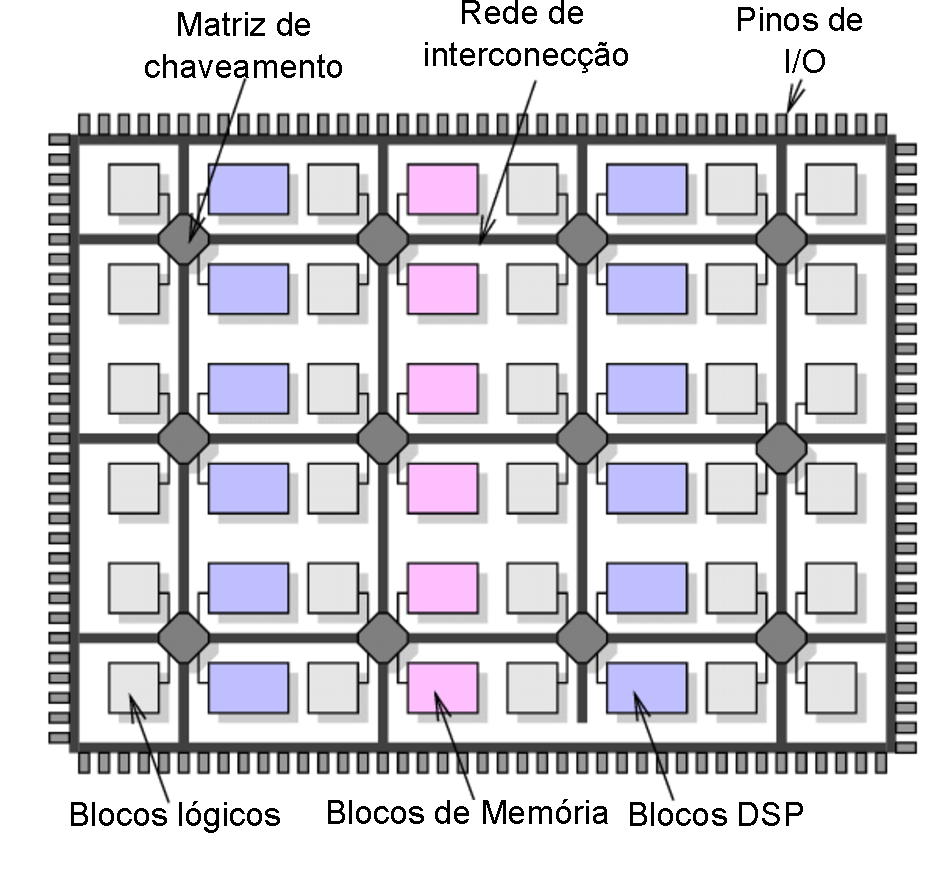
\includegraphics[width=0.6\linewidth]{figs/FPGA/FPGA.pdf}
    \caption{Arquitetura interna de um FPGA. Adaptado de \citeonline{langhammer2014design}.}
    \label{fig:FPGA_internal_architeture}
\end{figure}

Parte da lógica pode ser usada para instanciar um processador \textit{soft-core}, como o MicroBlaze da AMD, que executa código C sobre a lógica programável e se comunica com os demais blocos por barramentos AXI \cite{amd_ug984}. O projeto pode então ser particionado: funções de controle, comunicação e cálculo pouco crítico ficam em \textit{software}, enquanto as operações intensivas ou de latência estrita são implementadas em lógica dedicada.

\subsection{Fluxo de desenvolvimento}

A Figura~\ref{fig:FluxoDesenvolvimentoFPGA} resume o fluxo de desenvolvimento. Parte-se do algoritmo ou do modelo, que é otimizado (por exemplo, quantizado) e descrito em HDL ou em C/C++ para síntese de alto nível (\textit{High-Level Synthesis}, HLS). Na HLS, a ferramenta converte o código C em um circuito, e o projetista orienta o paralelismo por diretivas, como \textit{pipeline} e desenrolamento de laços \cite{cong2011hls,amd_ug1399}. Seguem a síntese lógica, que mapeia o projeto em LUTs, \textit{flip-flops}, DSPs e BRAMs, o posicionamento e roteamento (\textit{place \& route}) e a análise estática de temporização, que verifica se todos os caminhos cumprem o período de \textit{clock}. O fluxo é iterativo: os relatórios de recursos e de temporização e a verificação por simulação e em \textit{hardware} realimentam as etapas anteriores \cite{amd_ug900}.

\begin{figure}[htbp]
    \centering
    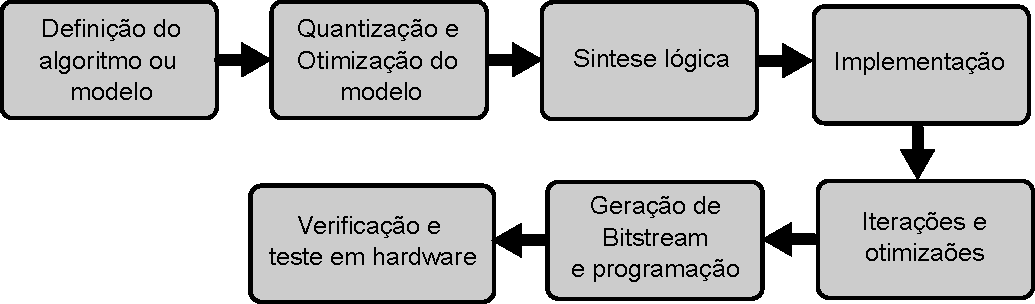
\includegraphics[width=0.75\linewidth]{figs/FPGA/FluxoOtimização.pdf}
    \caption{Fluxo de desenvolvimento e otimização de projetos em FPGA. Fonte: o autor.}
    \label{fig:FluxoDesenvolvimentoFPGA}
\end{figure}

\subsection{Quantização}

A técnica de otimização mais usada para executar redes neurais em FPGAs é a quantização: pesos e ativações deixam de ser representados em ponto flutuante de 32 bits e passam a inteiros de 8 bits ou menos, o que reduz memória, DSPs e lógica, com perda de acurácia em geral pequena \cite{jacob2018,nagel2021}. Na quantização afim, um valor real \(r\) é representado por um inteiro \(q\) com escala \(s\) e ponto zero \(z\),
\begin{equation}
	r \approx s\,(q - z), \qquad q = \mathrm{clip}\!\left(\mathrm{round}(r/s) + z,\; q_{\min},\; q_{\max}\right),
	\label{eq:quantizacao}
\end{equation}
e, na forma simétrica (\(z=0\)), comum para os pesos, \(s = \max|r|/127\) em int8. Os produtos de uma camada densa são acumulados em 32 bits e reescalados para a camada seguinte, de modo que toda a inferência usa só aritmética inteira. A quantização pode ser aplicada após o treinamento ou simulada durante ele (\textit{quantization-aware training}). Outras técnicas, como poda de conexões, fusão de camadas, \textit{pipeline} e uso de memória local, complementam a quantização \cite{Shawahna2019,mouri2025optimizing}.

\subsection{MLP em FPGA para diagnóstico de falhas}
\label{subsection:MLP}

Há diversas implementações de MLPs em FPGA. Alguns trabalhos tratam do custo da implementação: estimativa de recursos antes da síntese \cite{kokkinis2025fast}, poda e quantização \cite{ron2022experimental}, funções de ativação adequadas ao \textit{hardware} \cite{si2020neural}, co-projeto automático da rede e do circuito \cite{colangelo2020automl} e arquiteturas em \textit{pipeline} \cite{bahoura2011fpga}. No diagnóstico de máquinas, \citeonline{garcia2025detection} classificam curtos-circuitos incipientes entre espiras de motores de indução com uma MLP alimentada por descritores estatísticos da corrente, com precisão de 93,18\,\%. \citeonline{gaona2025fpga} classificam distúrbios de qualidade de energia com uma MLP 3-6-6 em um Artix-7. \citeonline{shreejith2016} usam reconfiguração parcial em um Zynq para alternar entre uma rede de detecção e outra que substitui um sensor defeituoso, com latência abaixo de 1\,\(\mu\)s. Por fim, \citeonline{toumi2022fpga} extraem atributos de envelope da vibração e os classificam com uma MLP em ponto fixo em um Zynq-7000, atingindo 95\,\% de acurácia no tipo de falha e 89\,\% na severidade na base CWRU, com coerência entre simulação e \textit{hardware}.

Esses trabalhos partem de sinais de baixa taxa (corrente, tensão, vibração), e nenhum combina detecção de \textit{hits} de EA na lógica com uma MLP sobre os descritores resultantes, que é a proposta deste trabalho.
